In this chapter, we present our ongoing work of building a cloud-based distributed testing service for PaaS applications.  The foundation of the service is a parallelization algorithm for symbolic execution that is the first to demonstrate linear scalability up to hundreds of cluster nodes.

\section{The Opportunity of the Cloud Application Model}

Modern consumer software is increasingly relying on the ``cloud application'' model, where a browser- or mobile device-based client interacts with a functionally rich cloud service.
%
This model is prevalent in major systems like Facebook and GMail, as well as in smartphone and tablet ``apps'' like Instagram, Siri, or Dropbox.
%
For both developers and users, the economics are highly \mbox{attractive:} cloud-based applications offer ubiquitous access, transparent scaling, and easy deployment at low cost.

The hidden cost is that cloud apps introduce security, privacy, and availability risks. They store and process critical information remotely, so the impact of failures is higher in this model than for single-user desktop apps~\cite{web-failures-tr}.  This increases the importance of testing for cloud applications.

Rapid advances in development and deployment tools have significantly lowered the barrier to entry for developers, but these tools lack similarly advanced support for testing. Platform-as-a-service (PaaS) offerings, such as Google App Engine or Microsoft Azure, provide easy-to-use interfaces with automated deployment fully integrated into development environments.
%
However, testing tools for apps running on PaaS are still immature, test automation is limited, and developers are left with the laborious and error-prone task of manually writing large numbers of individual test cases.

Integration tests, which complement unit tests by checking that all the components of a fully deployed cloud application work together correctly, are especially tedious to write and set up in such an environment.
%
PaaS-based cloud applications typically use frameworks with a layered communication architecture and perform some processing at each of the layers. Writing a full integration test then requires to carefully craft an HTTP request that successfully passes through all application and framework layers and triggers the desired behavior, while being transformed from one representation to another at each step (e.g., from an HTTP request to JSON to language objects).

Spending precious developer time on testing for improving security and reliability is particularly unattractive in a viciously competitive environment.  Promoted by the ability to deploy virtually instantly and at low cost, the pressure is to use features to quickly acquire a large user base. Security and reliability testing is a long-term investment and does not pay off immediately, thus it is often deferred for later.
%
High-profile failures of cloud applications~\cite{bugs-linkedin,bugs-gmail} are thus likely to become a common occurrence, unless we can make testing easy and cheap.

We argue that {\em testing} must become at least as easy as {\em deploying} a new app. PaaS has made the latter easy, leaving the former just as hard to do as before.  A dedicated testing service must therefore become an integral component of PaaS.
%
Recent commercial test automation systems (CloudBees, Skytap, SOASTA, etc.) relieve developers of managing their own test infrastructure, but still require them to write test suites; we aim to further relieve developers of having to write individual tests.
%
Just as modern PaaS APIs spare developers from having to manage the building blocks of their applications, so should they spare developers from manually writing test cases, and instead offer means to automatically test apps based on only minimal input from developers.

Recent progress in automated test case generation~\cite{klee,godefroid:fuzz,tillmann-pex} takes an important step in this direction.  For a typical PaaS application like the example in Figure~\ref{fig:running-example}, a test case generator could use \textit{symbolic execution} (a path-based program analysis) to automatically find HTTP packets that drive the execution to different parts of the code.
%
\begin{figure}
  \centering
  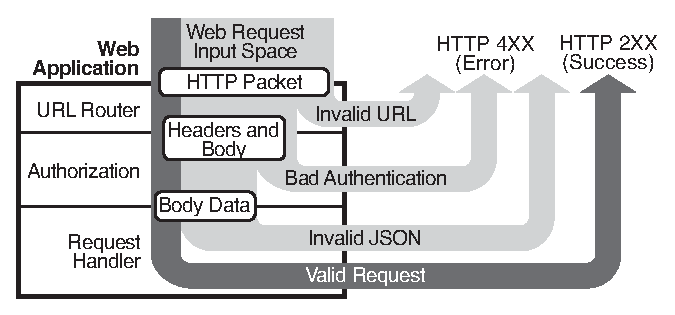
\includegraphics[width=3.1in]{figures/paas/web-flow}
  \caption{A sample cloud application.  Clients communicate with the server through web requests that traverse several layers inside the server before reaching the request handler logic.  From the total input space, most possible requests trigger errors in one of the processing layers (light arrows).  Only a small fraction of requests successfully traverses all layers and is handled inside the app (dark arrow).}
  \label{fig:running-example}
  \vspace{5pt}
\end{figure}
%
Unfortunately, these tools are not (yet) a good fit for cloud apps: the number of execution paths successfully crossing all application layers is dwarfed by the vast number of possible error paths (dark vs.~light arrows in Figure~\ref{fig:running-example}).  Yet, most error paths are irrelevant to testing the high-level logic of the app itself (i.e., the innermost layer), because they test code that is part of the PaaS.

We propose \textit{layered parameterized tests} (LPTs) for integration testing of PaaS-based cloud applications (Section~\ref{sec:paas:abstractions}). LPTs describe families of integration tests (in the spirit of parameterized unit tests~\cite{tillmann-puts}) across several application layers. We rely on developer-provided \textit{onion objects} to describe the layering of the data abstractions in the application; onion objects encode the multiple interpretations of input data as, e.g., an HTTP request, a JSON object, etc.
%
For the automatic generation of thorough test cases from LPTs, we introduce \emph{layered symbolic execution} (LSE), an automated program analysis that is tailored for the layered structure of cloud applications (Section~\ref{sec:paas:layeredsymbex}).
%
Finally, we present a design and early prototype for a PaaS-integrated testing service based on LSE~(Section~\ref{sec:paas:fedsymbex}).

\section{A PaaS Test Interface}
\label{sec:paas:abstractions}

We propose an automated testing service integrated in PaaS.  Developers write layered parameterized tests (LPTs) and upload them with the cloud application to be executed by the test service.  The service uses LPTs to automatically generate application inputs (e.g., web requests and persistent data) that exercise the application layers of interest.  The developer writes LPTs by specifying the structure of the application inputs and a target property to be checked.

\paragraph{Developer Workflow}

\begin{figure}
  \centering
  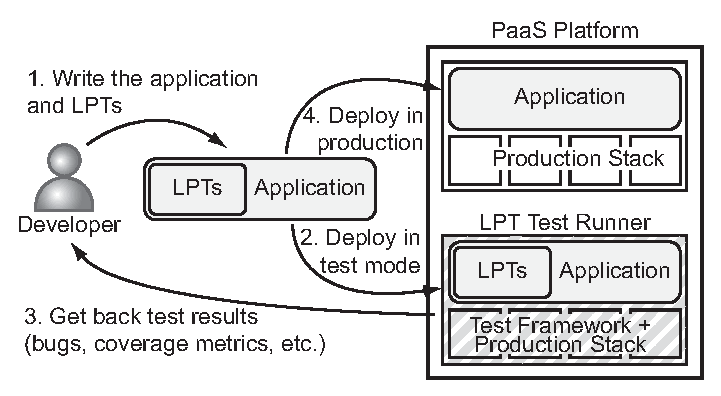
\includegraphics[width=3.1in]{figures/paas/developer-flow}
  \caption{Development flow for using a PaaS-integrated testing
    service.}
  \label{fig:development-flow}
\end{figure}

Figure~\ref{fig:development-flow} illustrates the workflow of a developer using our testing service.
%
The developer writes layered parameterized tests using a platform-provided testing API (step 1). She then deploys the app in test mode, which invokes the LPT test runner of the PaaS (step 2). This test runner is responsible for generating and running the individual test cases from the LPT, and it returns test results back to the developer (step 3). The develop-deploy-test cycle continues until the code is ready to be deployed in production (step 4).

% Might be misleading - the onion tests are much more powerful
% , and existing xUnit tests can be converted to onion tests.

%---------------------------------------------------------------------------
\paragraph{Layered Parameterized Tests}

An LPT specifies a family of executions (or, equivalently, classes of inputs) plus a set of properties (expressed as assertions) that are expected to hold for all these executions.
%
The specified family of executions can be large or even infinite; still, the test runner can often efficiently check whether the property is guaranteed to hold for the entire family (we give more details on the symbolic execution-based mechanism in Section~\ref{sec:paas:layeredsymbex}).  A traditional unit test can be seen as a special case of an LPT for which the input is fixed and any provided assertions are checked on a single execution only.

\begin{figure}
  \centering
  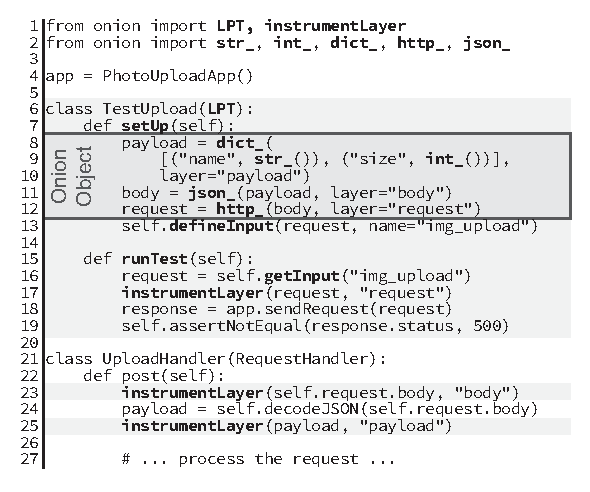
\includegraphics[width=3.2in]{figures/paas/overlay}
  \caption{An LPT example in Python for a photo management application.  Highlighted code is the test code written by developers.  Names in bold denote the LPT-specific API added to the standard Python unit test framework.}
  \label{fig:test-lpt}
\end{figure}

\looseness=-1 LPTs are defined by developers using a platform-provided API in the implementation language of the application (e.g., Python).  The testing API builds on the popular xUnit testing paradigm~\cite{xunit} and extends it with constructs to specify the structure of families of application inputs.  The API is easily integrated with existing testing fixtures and frameworks that developers use today.

We illustrate the structure of an LPT and how it is used by the test runner using the example LPT \codebit{TestUpload} shown in Figure~\ref{fig:test-lpt}, which tests the upload functionality of a photo management application.  Under the \codebit{/upload} URL, the application accepts POST requests containing a JSON-encoded dictionary describing photo information.  Figure~\ref{fig:http-packet} shows an example HTTP request for the application.

We assume that the app follows the structure given in Figure~\ref{fig:running-example}, that it is written in Python using a popular web framework like Django~\cite{py-django} or WebApp~\cite{webapp2}, and that it is deployed on a PaaS infrastructure like Google App Engine~\cite{google-gae} or Heroku~\cite{heroku}.  The web framework takes care of dispatching any POST request to the \codebit{/upload} application URL to the \codebit{post} method of the \codebit{UploadHandler} class (lines 21--27).
%
The \codebit{TestUpload} LPT checks that, for arbitrary upload requests, the server never returns an internal error (HTTP 500) in its response.

\begin{figure}
  \centering
  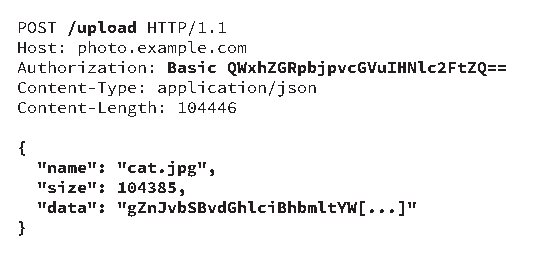
\includegraphics[width=3in]{figures/paas/http-packet}
  \caption{An example HTTP request for the upload feature of the photo
    management application.  The text in bold denotes input processed
    by the application at various layers.}
  \label{fig:http-packet}
\end{figure}

The test runner uses the LPT to automatically generate application
input according to the following procedure:

\begin{enumerate}
% Step 1
\item The test runner invokes the \codebit{setUp} method (line~7),
  which declares the application inputs and their structure as
  \emph{onion objects} (described below) using the
  \codebit{defineInput} call at line~13.
% Step 2
\item Based on the onion objects, the test runner generates a default
  input for the application.
% Step 3
\item The test runner invokes \codebit{runTest}, which retrieves the
  concrete input generated by the test runner with a call to
  \codebit{getInput} (line~16).  In our example, the input is a web
  request, which is then sent to the application (line~18).  Behind
  the scenes, the web framework dispatches the request to the
  \codebit{post} method of \codebit{UploadHandler} (line~22).  When
  the handler finishes handling the request, a response object with a
  status code and body is returned.  In our example, the LPT checks
  that no internal error (HTTP 500) occurred during request handling
  (line~19).
% Step 4
\item Based on the information collected during the execution of
  \codebit{runTest} (described below), the test runner uses the onion
  objects to generate a new application input (available to the LPT
  through the \codebit{getInput} call) and goes back to step 3 for a
  new iteration.  
%
  Any assertion failures triggered by the generated inputs are
  reported to the developers.
\end{enumerate}
%
Note that the generation and execution of multiple inputs is well
suited for parallelization across multiple nodes in the cloud. This
allows to leverage the availability of additional nodes to reduce the
total testing time.

The test runner uses symbolic execution to generate new inputs (described in more detail in Section~\ref{sec:paas:layeredsymbex}). To generate inputs that exercise the application at specific layers, the test runner needs:
\begin{itemize}
\item the unwrapped application inputs for the current execution at the different application layers, provided by developers through annotations in the application source code; and
\item information about the input structure, provided by the LPT's onion objects.
\end{itemize}

\paragraph{Annotating Application Layers}

A web request traverses several processing layers in an application.  First, it is received as an HTTP packet string; second, it is decoded into a URL, a set of headers, and request a body; third, the body contents is decoded and processed. Depending on the application framework, processing can involve additional layers, e.g., for converting JSON representations to language objects.

The application layers process data at corresponding layers of the input data (the bold parts of the HTTP request in Figure~\ref{fig:http-packet}). For instance, the application typically maps the URL to a request handler, checks the headers for authentication information, and processes the body contents in the request handler code.

To expose the application input to the LPT as it is being processed at each layer, developers annotate the variables holding the input data structures in the application source code.  Three layers have been declared in Figure~\ref{fig:test-lpt}: the HTTP request at line~17, the request body at line~23, and the JSON payload extracted from the body at line~25.  The \codebit{instrumentLayer} call attaches a layer name to a variable. Similar to assertion statements, the call is active when executed as part of a test invocation, but disabled in production, where the LPTs are not used.  For a typical web stack, only about three layers have to be annotated for each request handler, keeping the required effort on the developer side low.


%---------------------------------------------------------------------------
\paragraph{Onion Objects}

An \emph{onion object} is a data structure that describes the representations of the application input as it traverses multiple processing layers.  The onion object (i) enables more convenient assertion-writing by directly exposing the data layers, and (ii) enables automated test generation to focus on specific layers of the application. Onion objects are needed to specify the application inputs for onion tests, but they can also be used to store output as the cloud application constructs a response in layers.

The framed area in Figure~\ref{fig:test-lpt} shows the onion object for our running example.  The structure consists of a set of \emph{onion nodes} (the identifiers ending in an underscore) connected in a nested structure.  There is one onion node for each layer and one for each input structure or value that is supposed to be generated automatically by the test engine.  The abstraction level is declared using the \codebit{layer} parameter passed to the node constructor and matches one of the layers annotated in the code.  Structures and values can be nested within the same layer.  For example, the dictionary structure on lines~8--10 has constant keys and wildcard values of type \codebit{str\_} and \codebit{int\_}, which mimic the standard string and integer types.

\paragraph{Checking Properties}

LPTs express application properties through standard xUnit assertion statements (line~19 in the example).  Through the dynamic test generation mechanism explained in Section~\ref{sec:paas:layeredsymbex}, the test runner actively attempts to generate inputs that cause an assertion to be violated. Each generated test input not failing the assertion serves as a witness for an entire equivalence class of inputs that cannot violate the assertion.
%
When an assertion does fail, the input that caused the failure is reported back to the developer.

To allow input variables at each layer to be used in assertions, each onion node offers a \codebit{value} property that refers to the value matched in the current test execution (not shown in the example).

%%%%%%%%%%%%%%%%%%%%%%%%%%%%%%%%%%%%%%%%%%%%%%%%%%%%%%%%%%%%%%%%%%%%%%%%%%%%%%%%


\section{Layered Symbolic Execution}
\label{sec:paas:layeredsymbex}

In this section, we introduce \emph{layered symbolic execution} (LSE), an LPT execution technique that focuses on covering a particular application layer.  LSE uses symbolic execution---a test case generation technique that observes the program structure---to generate inputs in the representation of the layer of interest (e.g., HTTP headers or a JSON payload).  Each generated layer-level input is then assembled back into application-level input based on the structure encoded in the onion object, in order to form an integration test case.

Na\"ive application of dynamic test generation to execute the LPT for a cloud app is of little use: First, the path exploration can end up exploring many different paths within the framework code, but might test only a single path within the application layer over and over again. Second, the path conditions will encode many branches due to the multiple layers of parsing logic, making symbolic execution of cloud apps prohibitively expensive. Third, if the exploration is unaware of the connections between abstraction layers, blindly negating just single branch conditions will produce many infeasible paths before finding a new valid test input.

\paragraph{LSE and Onion Objects}

LSE relies on onion objects to mark input variables as symbolic and generate new values based on the alternate path conditions.  To this end, each onion object exposes a number of operations:

\begin{itemize}
\item \codebit{instrument(var)} instruments the variable \codebit{var}
  for symbolic execution, i.e., injects a fresh symbolic input value
  in dynamic test generation.  The variable is expected to match the
  structure described by the onion object.
%
\item \codebit{reconstruct(var, val)} applies an assignment of value \codebit{val} to variable \codebit{var} that is demanded by the satisfying assignment representing a new path. In doing the assignment, the function performs the necessary modifications to other variables to respect the cross-layer invariants.
%
\item \codebit{getDefault()} returns a default value for the object node. It is used for generating the initial test case or any padding values required by invariants (e.g., changing the content length field of an HTTP request requires to extend the actual contents).
\end{itemize}

For example, applying the \codebit{instrument} method of a string onion object on a string variable in Python marks as symbolic the string length and the contents of the character buffer.  Then, during symbolic execution, the alternate path constraint yields new values for the length and for the buffer.  The \codebit{reconstruct} method takes both values and creates a new Python string object.

The reconstruction method is essential for enforcing the object and cross-layer invariants of the input structure.  For instance, the length of the reconstructed string would always match the size of its buffer (and avoid spurious overflows); the Content-length HTTP header would always match the size of the new request body, and so on.

\paragraph{LSE Algorithm}

LSE allows the test runner to focus on exploring paths inside inner application layers. Conceptually, LSE decouples the input layers to give the test runner the flexibility to freely explore an individual layer. When constructing a new application input, LSE reconnects the layers, taking care to respect cross-layer invariants (e.g., the value of a JSON field has to be present also in the HTTP packet).
%
The LSE algorithm proceeds along the following steps:
\begin{enumerate}
\item Generate an initial valid input (i.e., a web request) using the
  \codebit{getDefault} call on the root node.  The LPT can read this
  input by calling \codebit{getInput}.
%
\item Symbolically execute the program through the test (the
  \codebit{runTest} method), using symbolic inputs created by calling
  the \codebit{instrument} method on the onion object nodes
  corresponding to the layer of interest.  
%
  Any existing symbolic expressions for these variables (which
  implicitly encode the parsing logic) are overwritten in this step,
  effectively decoupling the input at the current layer from the
  previous ones.  This permits the symbolic execution engine to negate
  constraints inside the current layer without being constrained
  by the previous layers.
%
\item When the execution completes, negate a constraint in the path
  condition to obtain new values for the onion nodes.
%
\item Using the $\codebit{reconstruct}$ function of the onion object
  node, assemble the new values back into a new complete program input
  (e.g., the HTTP request) for the next iteration.
\end{enumerate}

\begin{figure}
  \centering
  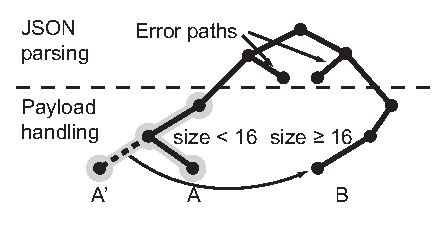
\includegraphics[width=2.4in]{figures/paas/layered-tree}
  \caption{Exploring an execution tree using layered symbolic
    execution.}
  \label{fig:layered-tree}
\end{figure}

Figure~\ref{fig:layered-tree} illustrates an execution tree explored in an iteration of LSE. Consider an initial input for the example in Figure~\ref{fig:test-lpt}, where the value of the $\codebit{size}$ field in the JSON request payload is $8$ (Path $A$ in the figure).
%
At step 2 of the algorithm, a symbolic value is injected for $\codebit{size}$, together with the rest of the onion object wildcard fields (the highlighted segment of Path $A$).  Now, if the tested path contains the conditional statement \codebit{if payload.size < 16}, the \codebit{then} branch of the statement is taken and the $\mathit{size} < 16$ constraint is recorded.  At the end of the execution (step 3), if this constraint is negated to $\mathit{size} \geq 16$, a new value for $\codebit{size}$ is generated, say $20$ (the alternate potential Path $A'$).  Then, at step 4, the \codebit{reconstruct} functions assembles the new values of all leaves into a new HTTP packet to be sent to the app, which will cause the \codebit{else} branch of the \codebit{if} statement to be taken in the next execution (Path $B$).  Note that Path $A'$ is not globally feasible and never explored, but only transiently used to produce the feasible Path $B$.

Compared to a solution that only marks the variables at the layers of interest as symbolic, LSE is superior in two ways: (1)~By obtaining the root input, it is able to run integration tests for a fully deployed application; (2)~LSE supports data structures of variable sizes, e.g., arrays whose lengths are symbolic values, by regenerating the input structure at each new iteration.

%%%%%%%%%%%%%%%%%%%%%%%%%%%%%%%%%%%%%%%%%%%%%%%%%%%%%%%%%%%%%%%%%%%%%%%%%%%%%%%%

\section{A Testing Platform for the Cloud}
\label{sec:paas:fedsymbex}

We deploy LSE inside a symbolic execution-aware virtual machine (the symbolic VM) that encapsulates the ``entire universe'' of the application, including the framework and even the language interpreter and operating system, enabling integration testing of the entire application stack.
%
The test-mode deployment then requires just the push of a button for the system to execute the layered parameterized tests, generate coverage statistics, and highlight any failing test cases.

This deployment model leverages the properties of PaaS in several
ways:
%
(1)~By hiding the testing VMs behind a service interface, the PaaS system can faithfully reproduce the exact environment of production VMs inside the testing VMs without exposing its internals.
%
(2)~The testing task can be transparently scaled across multiple VMs
by using parallel symbolic execution~\cite{cloud9}.
%
(3)~Since the application uses standard interfaces for accessing the PaaS components (storage, networking, etc.), the provider is able to substitute production-optimized implementations with testing-optimized stubs that offer a simplified behavior that is better suited to automated program analysis.

From the perspective of the PaaS provider, the test runner service consists of a set of symbolic VMs, operated separately from the production infrastructure.  When an application is deployed in test mode, one of the symbolic VMs is allocated for testing: the application code and tests are copied to the guest, and the LSE algorithm is invoked.

\paragraph{Architecture}

\begin{figure}
  \centering
  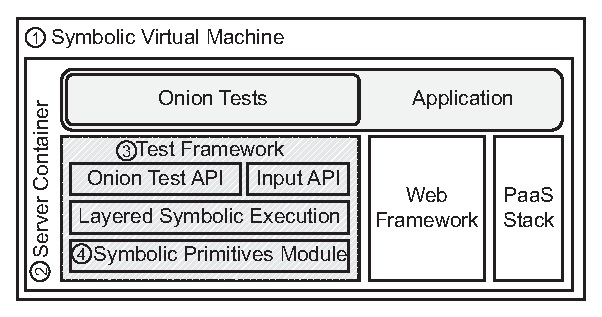
\includegraphics[width=3.1in]{figures/paas/symbolic-vm}
  \caption{The PaaS test runner service.}
  \label{fig:fse}
\end{figure}

Figure~\ref{fig:fse} illustrates the architecture of the symbolic VM
environment.  Inside the VM~\cI, all application components are
symbolically executed in the same low-level representation (e.g., x86
machine code or LLVM~\cite{llvm}).  The components execute inside
their own vanilla interpreters~\cII.  
%
The test framework~\cIII plays two roles: it implements (1) the APIs for LPTs and onion objects that developers use to write the testing code, and (2) the LSE algorithm that guides the test case generation.

\paragraph{Prototype}

We implemented a prototype of the symbolic VM that tests Python-based Google App Engine PaaS applications and is built on top of the S2E symbolic virtual machine.

In our implementation, the symbolic execution engine and the LSE logic live at different levels in the symbolic VM stack.
%
The symbolic execution engine operates with low-level abstractions such as memory bytes. It resides on the host level, as an S2E plugin that exposes the core symbolic execution primitives to the guest as S2E system calls, e.g., to allow marking memory buffers as symbolic.
%
The LSE algorithm operates on web application state (e.g., by accessing the onion objects), and is implemented in the guest as a native Python extension module.  We implemented LSE on top of WebTest~\cite{py-webtest}, a popular fixture library for testing Python web applications.
%
The resulting system is extensible to other languages with limited engineering effort: since the symbolic execution logic is provided at the host level, only the test framework component needs to be implemented in the cloud app language.

Early experiences with the prototype are encouraging: for the full application stack of a simple cloud app, our prototype generates a test case every few seconds.

%%%%%%%%%%%%%%%%%%%%%%%%%%%%%%%%%%%%%%%%%%%%%%%%%%%%%%%%%%%%%%%%%%%%%%%%%%%%%%%%

\section{Parallel Symbolic Execution in Cloud9}
\label{sec:paas:parsymbex}

Since the size of the execution tree is exponential in the number of branches, and the complexity of constraints increases as the tree deepens, state-of-the-art SEEs can quickly bottleneck on CPU and memory even for programs with just a couple \kloc.  We therefore build a parallel SEE that runs on a commodity cluster and enables ``throwing hardware at the problem.''

The key design goal is to enable individual cluster nodes to explore the execution tree independently of each other.  One way of doing this is to statically split the execution tree and farm off subtrees to worker nodes.  Alas, the contents and shape of the execution tree are not known until the tree is actually explored, and finding a balanced partition (i.e., one that will keep all workers busy) of an unexpanded execution tree is undecidable.  Besides subtree size, the amount of  memory and CPU required to explore a subtree is also undecidable, yet must be taken into account when partitioning the tree. Since the methods used so far in parallel model checkers~\cite{swarm,spin:multicore-modelchecking} rely on static partitioning of a finite state space, they cannot be directly applied to the present problem. Instead, \cnine partitions the execution tree {\em dynamically}, as the tree is being explored. 

%--------------------------------------------------
\paragraph{Dynamic Distributed Exploration}

\cnine consists of wor\-ker nodes and a load balancer (LB).  Workers run independent SEEs, based on \klee~\cite{klee}.  They explore portions of the execution tree and send statistics on their progress to the LB, which in turn instructs, whenever necessary, pairs of workers to balance each other's work load.  Encoding and transfer of work is handled directly between workers, thus taking the load balancer off the critical path.

The goal is to dynamically partition the execution tree such that the parts are {\em disjoint} (to avoid redundant work) and together they {\em cover} the global execution tree (for exploration to be complete).  We aim to minimize the number of work transfers and associated communication overhead.  A fortuitous side effect of dynamic partitioning is the transparent handling of fluctuations in resource quality, availability, and cost, which are inherent to large clusters in cloud settings.

\cnine operates roughly as follows: The first component to come up is the load balancer.  When the first worker node $W_1$ joins the \cnine cluster, it connects to the LB and receives a ``seed'' job to explore the entire execution tree.  When the second worker $W_2$ joins and contacts the LB, it is instructed to balance $W_1$'s load, which causes $W_1$ to break off some of its unexplored subtrees and send them to $W_2$ in the form of {\em jobs}.  As new workers join, the LB has them balance the load of existing workers.  The workers regularly send to the LB status updates on their load in terms of exploration jobs, along with current progress in terms of code coverage, encoded as a bit vector.  Based on workers' load, the LB can issue job transfer requests to pairs of workers in the form $\langle$~source worker, destination worker, \# of jobs~$\rangle$.  The source node decides which particular jobs to transfer.

\subsection{Worker-level Operation}
\label{sec:workerView}

A worker's visibility is limited to the subtree it is exploring locally.  As $W_i$ explores and reveals the content of its local subtree, it has no knowledge of what $W_j$'s ($i\ne j$) subtree looks like.  No element in the system---not even the load balancer---maintains a global execution tree.  Disjointness and completeness 
of the exploration (see Fig.~\ref{fig:architecture}) are ensured by the load balancing algorithm.

\begin{figure}[h!]
  \centering
  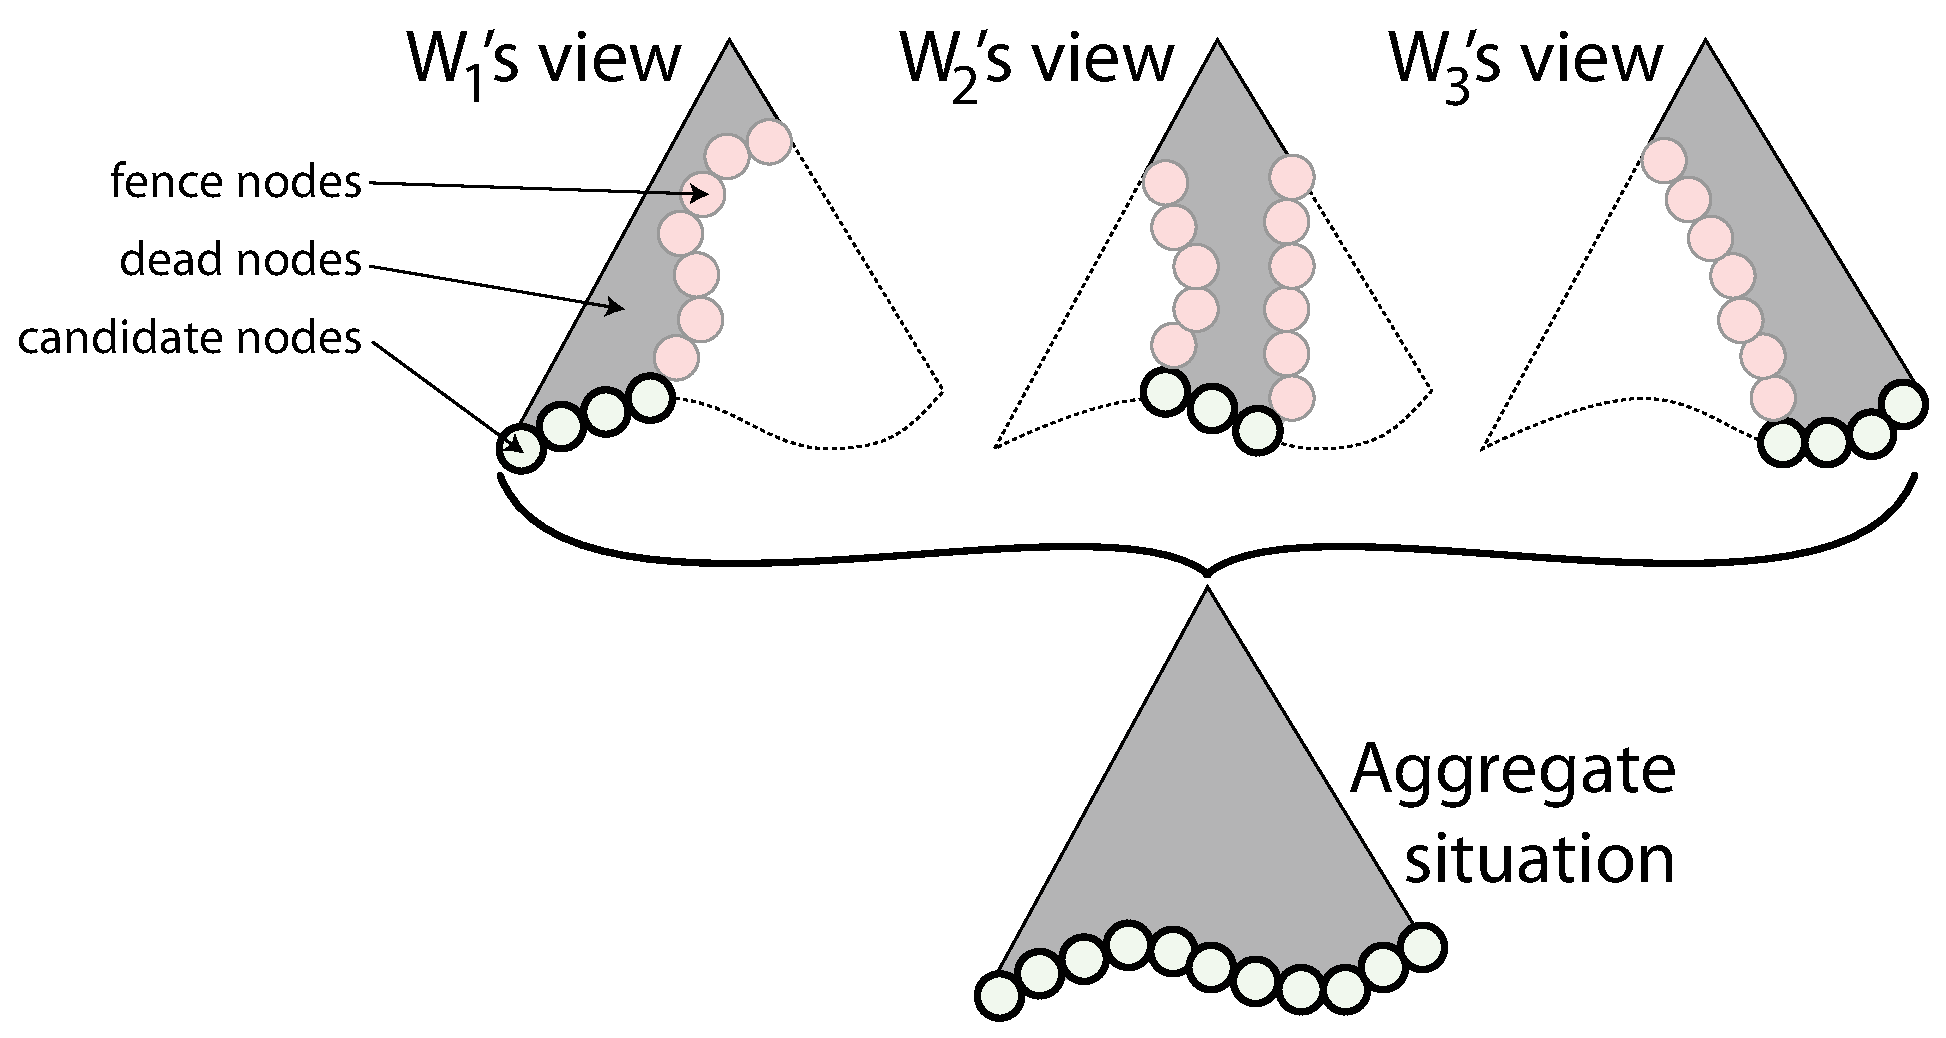
\epsfig{file=figures/parsymbex/architecture-parsymbex, height=1.7in}
  \caption{Dynamic partitioning of exploration in \cnine.}
 \label{fig:architecture}
\end{figure}

\newcommand{\dead}{dead\xspace}
\newcommand{\fence}{fence\xspace}
\newcommand{\candidate}{candidate\xspace}
\newcommand{\virtual}{virtual\xspace}
\newcommand{\materialized}{materialized\xspace}

As will be explained later, each worker has the root of the global execution tree.  The tree portion explored thus far on a worker consists of three kinds of nodes: (1) internal nodes that have already been explored and are thus no longer of interest---we call them {\em \dead} nodes; (2) {\em \fence} nodes that demarcate the portion being explored, separating the domains of different workers; and (3) {\em \candidate} nodes, which are nodes ready to be explored.  A worker exclusively explores \candidate nodes; it never expands \fence or \dead nodes.

Candidate nodes are leaves of the local tree, and they form the \emph{exploration frontier}.  The work transfer algorithm ensures that frontiers are disjoint between workers, thus ensuring that no worker duplicates the exploration done by another worker.  At the same time, the union of all frontiers in the system corresponds to the frontier of the global execution tree. The goal of a worker  $W_i$ at every step is to choose the next \candidate node to explore and, when a bug is encountered, to compute the inputs, thread schedule, and system call returns that would take the program to that bug.

%--------------------------------------------------
\paragraph{Worker-to-Worker Job Transfer}
\label{sec:workTransfer}

\newcommand{\wsrc}{\ensuremath{W_s}\xspace}
\newcommand{\wdst}{\ensuremath{W_d}\xspace}

When the global exploration frontier becomes poorly balanced across workers, the load balancer chooses a loaded worker \wsrc and a less loaded worker \wdst  and instructs them to balance load by sending $n$ jobs from \wsrc to \wdst.  In the extreme, \wdst is a new worker or one that is done exploring its subtree and has zero jobs left.  

\wsrc chooses $n$ of its \candidate nodes and packages them up for transfer to \wdst.  Since a \candidate node sent to another worker is now on the boundary between the work done by \wsrc and the work done by \wdst, it becomes a \fence node at the sender.  This conversion prevents redundant work.

A job can be sent in at least two ways: (1) serialize the content of the chosen node and send it to \wdst, or (2) send to \wdst the path from the tree root to the node, and rely on \wdst to ``replay'' that path and obtain the contents of the node.  Choosing one vs. the other is a trade-off between time to encode/decode and network bandwidth: option (1) requires little work to decode, but consumes bandwidth (the state of a real program is typically at least several megabytes), while encoding a job as a path requires replay on \wdst.  We assume that large commodity clusters have abundant CPU but meager bisection bandwidth,
so in \cnine we chose to encode jobs as the path from the root to the \candidate node.  As an optimization, we exploit common path prefixes: jobs are not encoded separately, but rather the corresponding paths are aggregated into a job tree and sent as such.

\begin{wrapfigure}{r}{1in}
\vspace{-5mm}
%
%\includegraphics[height=50mm]{new-diagrams/worker-tree-thumb}
\hspace{-10mm}\includegraphics[height=50mm]{figures/parsymbex/worker-tree-thumb}
%\caption{Example of a local worker tree.}
\vspace{-8mm}
\end{wrapfigure}

When the job tree arrives at \wdst, it is imported into \wdst's own subtree, and the leaves of the job tree become part of \wdst's frontier (at the time of arrival, these nodes may lie ``ahead'' of \wdst's frontier).  \wdst keeps the nodes in the incoming jobs as {\em \virtual} nodes, as opposed to {\em \materialized} nodes that reside in the local subtree, and replays paths only lazily.  A \materialized node is one that contains the corresponding program state, whereas a \virtual node is an ``empty shell'' without corresponding program state.  In the common case, the frontier of a worker's local subtree contains a mix of \materialized and \virtual nodes, as shown in the diagram above.

As mentioned earlier, a worker must choose at each step which \candidate node to explore next---this choice is guided by a {\em strategy}.  Since the set of \candidate nodes now contains both \materialized and \virtual nodes, it is possible for the strategy to choose a \virtual node as the next one to explore.  When this happens, the corresponding path in the job tree is replayed (i.e., the symbolic execution engine executes that path); at the end of this replay, all nodes along the path are \dead, except the leaf node, which has converted from \virtual to \materialized and is now ready to be explored.  Note that, while exploring the chosen job path, each branch produces child program states; any such state that is not part of the path is marked as a \fence node, because it represents a node that is being explored elsewhere, so \wdst should not pursue it.

\paragraph{Summary}

\newcommand{\status}{\ensuremath{\mathrm{status}}\xspace}
\newcommand{\alive}{\ensuremath{\mathrm{life}}\xspace}

A node $N$ in $W_i$'s subtree has two attributes, $N^{\status} \in$\{\materialized, \virtual\!\} and $N^{\alive} \in$\{\candidate, \fence, \dead\!\}.  A worker's frontier $F_i$ is the set of all \candidate nodes on worker $W_i$.  The worker can only explore nodes in $F_i$, i.e., \dead nodes are off-limits and so are \fence nodes, except if a \fence node needs to be explored during the replay of a job path.  The union $\cup F_i$ equals the frontier of the global execution tree, ensuring that the aggregation of worker-level explorations is complete.  The intersection $\cap F_i = \emptyset$, thus avoiding redundancy by ensuring that workers explore disjoint subtrees.  Fig.~\ref{fig:transitions} summarizes the life cycle of a node.

\begin{figure}[h!]
  \centering
  \hspace{-4mm}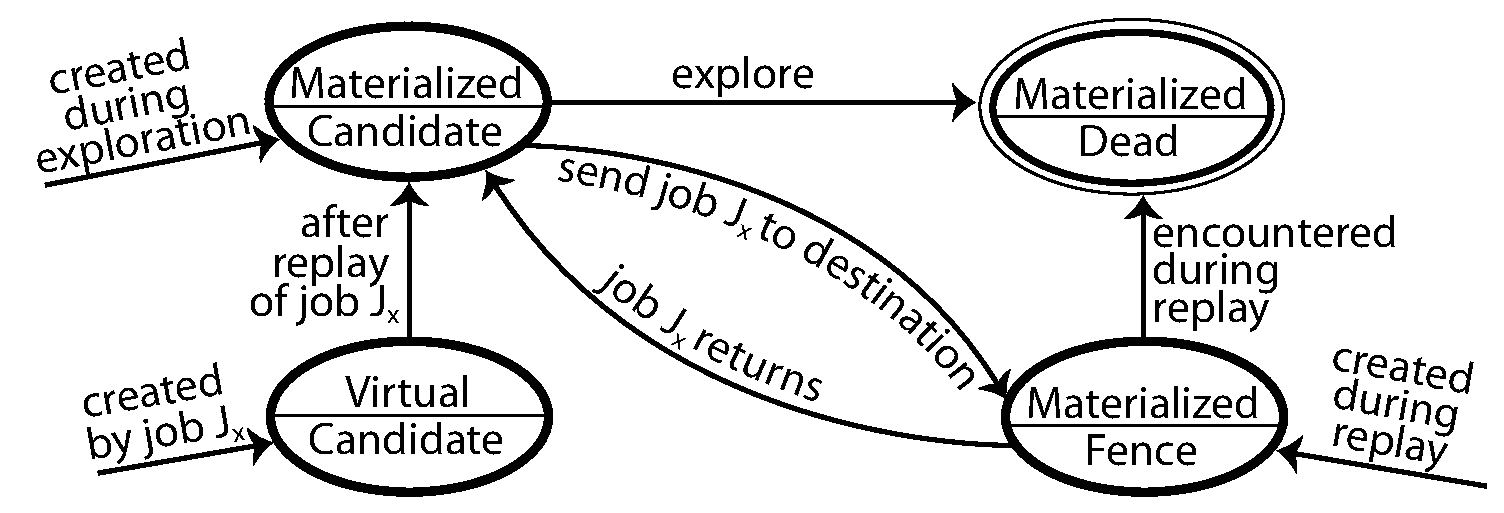
\epsfig{file=figures/parsymbex/node-transitions, width=3.4in}
  \caption{Transition diagram for nodes in a worker's subtree.}
 \label{fig:transitions}
\end{figure}

As suggested in Fig.~\ref{fig:transitions}, once a tree node is \dead, it has reached a terminal state; therefore, a dead node's state can be safely discarded from memory.  This enables workers to maintain program states only for \candidate and \fence nodes.

%%%%%%%%%%%%%%%%%%%%%%%%%%%%%%%%%%%%%%%%%%%%%%%%%%%%%%%%%%%%%%%%%%%%%%%%%%%%%%%%

\subsection{Cluster-level Operation}
\label{sec:loadBalancing}

\paragraph{Load Balancing}

When jobs arrive at \wdst, they are placed conceptually in a queue; the \emph{length} of this queue is sent to the load balancer periodically.  The LB ensures that the worker queue lengths stay within the same order of magnitude.  The balancing algorithm takes as input the lengths $l_i$ of each worker $W_i$'s queue $Q_i$.  It computes the average $\bar{l}$ and standard deviation $\sigma$ of the $l_i$ values and then classifies each $W_i$ as underloaded ($l_i < max \{ \bar{l}-\delta \cdot \sigma, 0 \}$), overloaded ($l_i > \bar{l} + \delta \cdot \sigma$), or OK otherwise; $\delta$ is a constant factor.  The $W_i$ are then sorted according to their queue length $l_i$ and placed in a list.  LB then matches underloaded workers from the beginning of the list with overloaded workers from the end of the list.  For each pair $\langle W_i,W_j \rangle$, with $l_i < l_j$, the load balancer sends a job transfer request to the workers to  move $(l_j - l_i)/2$ \candidate nodes from $W_j$ to $W_i$.


%===========================================================================
\paragraph{Coordinating Worker-level Explorations}
\label{sec:globalStrategy}

Classic symbolic execution relies on heuristics to choose which state on the frontier to explore first, so as to efficiently reach the chosen test goal (code coverage, finding a particular type of bug, etc.). In a distributed setting, local heuristics must be coordinated across workers to achieve the global goal, while keeping communication overhead at a minimum. What we have described so far ensures that eventually all paths in the execution tree are explored, but it provides no aid in focusing on the paths desired by the global strategy.  In this sense, what we described above is a \emph{mechanism}, while the exploration strategies represent the \emph{policies}.

Global strategies are implemented in \cnine using its interface for building {\em overlays} on the execution tree structure.  We used this interface to implement distributed versions of all strategies that come with \klee~\cite{klee}; the interface is also available to \cnine users.  Due to space limitations, we do not describe the strategy interface further, but provide below an example of how a global strategy is built.

A coverage-optimized strategy drives exploration so as to maximize coverage~\cite{klee}.  In \cnine, coverage is represented as a bit vector, with one bit for every line of code; a set bit indicates that a line is covered.  Every time a worker explores a program state, it sets the corresponding bits locally. The current version of the bit vector is piggybacked on the status updates sent to the load balancer.  The LB maintains the current global coverage vector and, when it receives an updated coverage bit vector, {\small OR}s it into the current global coverage.  The result is then sent back to the worker, which in turn {\small OR}s this global bit vector into its own, in order to enable its local exploration strategy to make choices consistent with the global goal.  The coverage bit vector is an example of a \cnine overlay data structure.

\subsection{Scalability Evaluation}
\label{sec:scalability}

We evaluate \cnine\ using two metrics:
\begin{enumerate}
\item The time to reach a certain goal (e.g., an exhaustive path exploration, or a fixed coverage level)---we consider this an \emph{external} metric, which measures the performance of the testing platform in terms of its end results.
\item The useful work performed during exploration, measured as the number of useful (non-replay) instructions executed symbolically. This is an \emph{internal} metric that measures the efficiency of \cnine's internal operation. 
%Useful instructions also mean that the shared prefixes of any two paths in the program are considered only once, according by this metric. 
\end{enumerate}

A cluster-based symbolic execution engine \emph{scales} with the number of workers if these two metrics improve proportionally with the number of workers in the cluster.

\paragraph{Time Scalability} We show that \cnine\ scales linearly by achieving the same testing goal proportionally faster as the number of workers increases. We consider two scenarios.

First, we measure how fast \cnine\ can exhaustively explore a fixed number of paths in the symbolic execution tree.  For this, we use a symbolic test case that generates all the possible paths involved in receiving and processing two symbolic messages in the memcached server.  Fig.~\ref{fig:scalab-time-vs-workers} shows the time required to finish the test case with a variable number of workers: every doubling in the number of workers roughly halves the time to completion.  With 48 workers, the time to complete is about 10 minutes; for 1 worker,  exploration time exceeds our 10-hour limit on the experiment.  

%The results of the experiment show an important aspect: while the path explosion problem cannot simply be solved by thowing more hardware at it, the size of the problems for which symbolic execution can be useful today are within the range in which a parallel symbolic execution engine can make a significant difference.

\begin{figure}[h!]
  \centering
  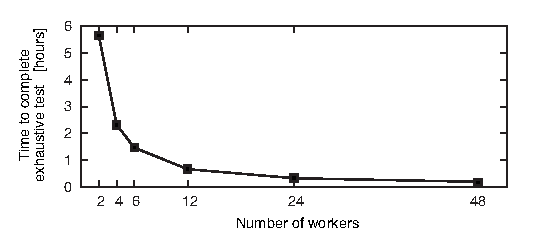
\epsfig{file=figures/evaluation/scalab-time-vs-workers-edited.eps, width=2.9in}
  \caption{\cnine\ scalability in terms of the time it takes to exhaustively complete a symbolic test case for memcached.}
  \label{fig:scalab-time-vs-workers}
\end{figure}

\begin{figure}[h!]
  \centering
  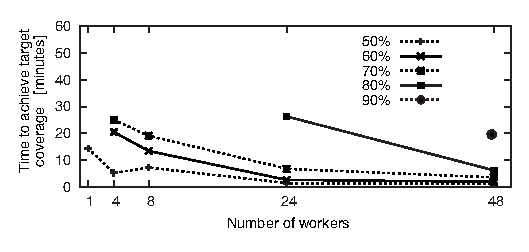
\epsfig{file=figures/evaluation/scalab-time-vs-workers-cov-printf-edited.eps, width=2.9in}
  \caption{\cnine\ scalability in terms of the time it takes to obtain a target coverage level when testing \codebit{printf}.}
  \label{fig:scalab-time-vs-workers-cov}
\end{figure}

\begin{figure}[t!]
  \centering
  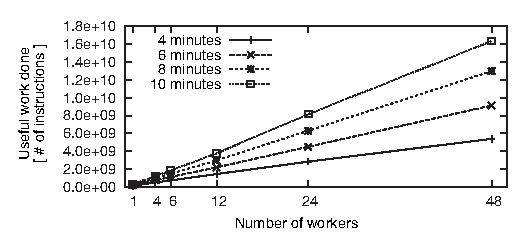
\epsfig{file=figures/evaluation/scalab-thr-cpu-vs-workers-memcached-edited.eps, width=2.9in} \\
  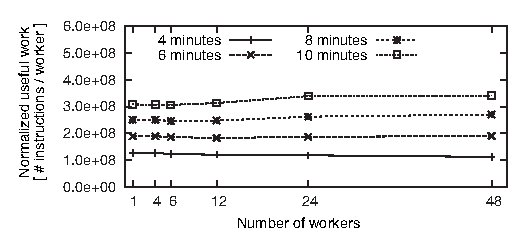
\epsfig{file=figures/evaluation/scalab-thr-cpu-perc-vs-workers-memcached-edited.eps, width=2.9in}
  \caption{\cnine\ scalability in terms of useful work done for four different running times when testing memcached.}
  \label{fig:scalab-memcached}
\end{figure}

\begin{figure}[h!]
  \centering
  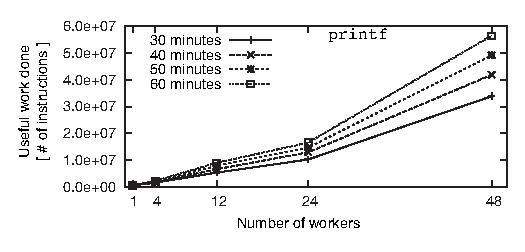
\epsfig{file=figures/evaluation/scalab-thr-cpu-vs-workers-edited.eps, width=2.9in} \\
  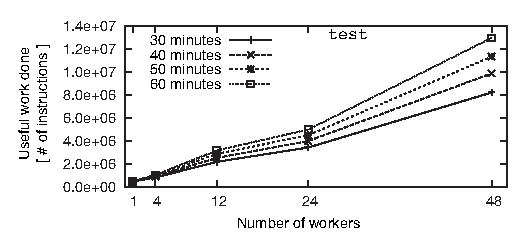
\epsfig{file=figures/evaluation/scalab-thr-cpu-vs-workers-test-edited.eps, width=2.9in}
  \caption{\cnine's useful work on \codebit{printf} (top) and \codebit{test} (bottom) increases roughly linearly in the size of the cluster.}  
  \label{fig:scalab}
\end{figure}

Second, we measure the time it takes \cnine\ to reach a fixed coverage level for the \codebit{printf} UNIX utility.  \codebit{printf} performs a lot of parsing of its input (format specifiers), which produces complex constraints when executed symbolically.   Fig.~\ref{fig:scalab-time-vs-workers-cov} shows that the time to achieve a coverage target decreases proportionally with the number of added workers.  The low 50\% coverage level can be easily achieved even with a sequential SEE (1-worker \cnine). However, higher coverage levels require more workers, if they are to be achieved in a reasonable amount of time; e.g., only a 48-worker \cnine is able to achieve  $90\%$ coverage.  The anomaly at 4 workers for 50\% coverage is due to high variance; when the number of workers is low, the average (5$\pm$4.7 minutes over 10 experiments) can be erratic due to the random choices in the random-path search strategy.

\paragraph{Work Scalability} We now consider the same scalability experiments from the perspective of useful work done by \cnine: we measure both the total number of instructions (from the target program) executed during the exploration process, as well as normalize this value per worker. This measurement indicates whether the overheads associated with parallel symbolic execution impact the efficiency of exploration, or are negligible. Fig.~\ref{fig:scalab-memcached} shows the results for memcached, confirming that \cnine scales linearly in terms of useful work done (top graph).  The average useful work done by a worker (bottom graph) is relatively independent of the total number of workers in the cluster, so adding more workers improves proportionally \cnine's results.

In Fig.~\ref{fig:scalab} we show the results for \codebit{printf} and \codebit{test}, UNIX utilities that are an order of magnitude smaller than memcached. We find that the useful work done scales in a similar way to memcached, even though the three programs are quite different from each other (e.g., \codebit{printf} does mostly parsing and formatting, while memcached does mostly data structure manipulations and network I/O).


In conclusion, \cnine scales linearly with the number of workers, both in terms of the time to complete a symbolic testing task and in terms of reaching a target coverage level.  % As far as the performed work is concerned, we observe that worker efficiency increases as the total number of workers in the system increases.


\iffalse
\subsection{Utility of Load Balancing}
\label{sec:profiling}
 
In this section we explore the utility of dynamic load balancing.  Consider the example of exhaustively exploring paths with two symbolic packets in memcached, using 48 workers, but this time from a load balancing perspective. Fig.~\ref{fig:scalab-load-balancing} shows that load balancing events occur frequently, with \linebreak 3--6\% of all states in the system being transferred between workers in almost every 10-second time interval.

\begin{figure}[h!]
  \centering
  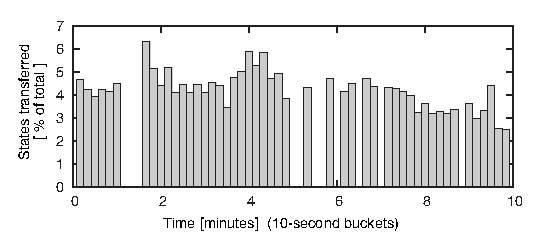
\epsfig{file=figures/evaluation/scalab-load-balancing-edited.eps, width=3in}
  \caption{The fraction of total states (candidate nodes) transferred between workers during symbolic execution.}
  \label{fig:scalab-load-balancing}
\end{figure} 

To illustrate the benefits of load balancing, we disable it at various moments in time and then analyze the evolution of total useful work done. Fig.~\ref{fig:scalab-static-balancing} shows that the elimination of load balancing at any moment during the execution significantly affects the subsequent performance of exploration due to the ensuing imbalance.  This demonstrates the necessity of taking a dynamic approach to parallel symbolic execution, instead of doing mere static partitioning of the execution tree.

\begin{figure}[h!]
  \centering
  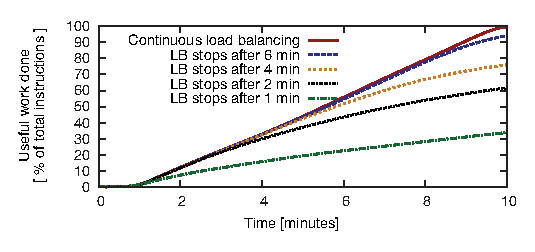
\epsfig{file=figures/evaluation/scalab-static-balancing-edited.eps, width=3in}
  \caption{Instruction throughput of \cnine\ with load balancing disabled at various points during the exhaustive test.}
  \label{fig:scalab-static-balancing}
  \vspace{-0.5cm}
\end{figure}

\subsubsection{Case Study \#1: UNIX Utilities}
\label{sec:coreutils}

\topic{\klee is an excellent tool for testing command-line programs, in particular \unix utilities.}  It does not tackle more complex systems, like the ones in Table~\ref{table:tested}, mainly due to path explosion (since \klee is a single-node engine) and insufficient environment support.  We cannot compare \cnine to \klee on parallel and distributed systems, but we can compare on the Coreutils suite of \unix utilities~\cite{coreutils}.

We run \klee on each of the 96 utilities for 10 minutes, and then  run a 12-worker \cnine on each utility for 10 minutes. Fig.~\ref{fig:coreutils-cov} reports the average coverage increase obtained with \cnine over 7 trials, using \klee's 7-trial average results as a baseline; the experiment totals $2 \times 7 \times 96 \times 10 = 13,440$ minutes $>$ 9 days.  The increase in coverage is measured as {\em additional} lines of code covered, expressed as a percentage of program size (i.e., we do not report it as a percentage of the baseline, which would be a higher number).

\topic{\cnine covers up to an additional $40\%$ of the target programs, with an average of $13\%$ additional code covered across all Coreutils.}  In general, improving coverage becomes exponentially harder as the base coverage increases, and this effect is visible in the results: a $12\times$ increase in hardware resources does not bring about a $12\times$ increase in coverage.  Our results show that \cnine allows ``throwing hardware'' at the automated testing problem, picking up where \klee left off.  In three cases, \cnine achieved $100\%$ coverage in 10 minutes on real-world code.  This experiment does not aim to show that \cnine is a ``better'' symbolic execution engine than \klee---after all, \cnine is based on \klee---but rather that \cnine-style parallelization can make existing symbolic execution engines more powerful.

The way we compute coverage is different from~\cite{klee}---whereas \klee was conceived as an automated {\em test generator}, \cnine is meant to {\em directly test} software. Thus, we measure the number of lines of code tested by \cnine, whereas \cite{klee} reports numbers obtained by running the concrete test cases generated by \klee.  Our method yields more-conservative numbers because a test generated by \klee at the end of an incomplete path (e.g., that terminated due to an environment failure) may execute further than the termination point when run concretely.

\begin{figure}[h!]
  \centering
  \label{fig:coreutils-final-cov}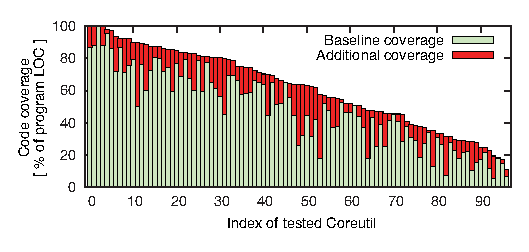
\epsfig{file=figures/evaluation/coreutils-cov-edited.eps, width=3.2in} \\
  \label{fig:coreutils-delta-cov}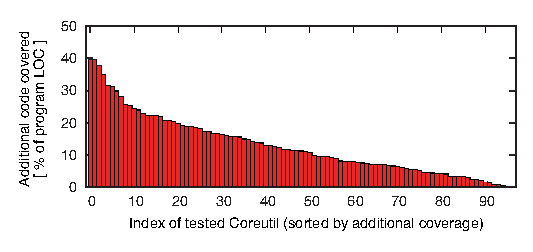
\epsfig{file=figures/evaluation/coreutils-delta-cov-edited.eps, width=3.2in}
  \caption{\cnine coverage improvements on the 96 Coreutils (1-worker \cnine vs. 12-worker \cnine).}
  \label{fig:coreutils-cov}
\end{figure}
\fi


%%% Local Variables: 
%%% mode: latex
%%% eval: (visual-line-mode)
%%% fill-column: 1000000
%%% TeX-master: "main"
%%% End:
